\chapter{Advances in Geometric Bayesian Inference} \label{ch:mcmc}
In this chapter we propose using the geometry of the log target density in two different inference methods for drawing samples. The first one (Paper I) is a distributional approximation to the target distribution using a generalization of the Laplace approximation. The second one (Paper II) uses MCMC and generalizes the hit-and-run slice-sampler to a particular Riemannian setting in which geodesics are not closed form. 

This chapter starts by introducing common elements between our contributions. These elements rely on the notions of Riemannian geometry presented in Chapter~\ref{ch:background}.
We introduce choices for the metric tensor, the volume, the Hausdorff density, and discuss the numerical computation of the exponential map. Then, we present the Riemannian Laplace approximation with the Fisher metric and the geodesic slice sampler for multimodal distributions with strong curvature. 

\paragraph{Motivation}
Equipping the space with a non Euclidean geometry increases computational complexity (dependent on the metric choice), but can lead to higher quality samples. In particular, it enables exploration of curved regions of the parameter space and better captures multimodal distributions compared to Euclidean methods.

\section{Choice of metric tensor} \label{sec:geometric_tools}

We consider a target density $p(\boldsymbol{x})$ defined over $\mathbb{R}^D$ with respect to the Lebesgue measure. We give the Euclidean space the Riemannian metric $\mathbf{G}(\boldsymbol{x})$. Once the metric is fixed it determines the local geometry of the space and determines the geometric objects used in this chapter such as geodesics, logarithm map and volume elements.

\subsection{Riemannian metrics}
The Riemannian metrics we consider in this chapter depend on the probabilistic model, through the log density $\log p(\boldsymbol{x})$, and each of them leads to a different geometry. Next we introduce the metric choices,  and give the corresponding inverse, determinant and Christoffel symbols needed for geodesic computations.


\paragraph{Euclidean metric}
Let us present Euclidean space using the same tools as more general cases. Euclidean space is equipped with a constant metric, 
\begin{equation*}
 \mathbf{G}(\boldsymbol{x}) = \mathbf{I}_D.
\end{equation*}
The Christoffel symbols vanish $\Gamma_{ij}^k=0$ for all $i,j,k=1,\ldots,D$ and the exponential and logarithm map are, for $\boldsymbol{x},\boldsymbol{y} \in \mathbb{R}^D$ and $\boldsymbol{v} \in T_{\boldsymbol{x}} \mathbb{R}^D \cong \mathbb{R}^D$,
\begin{equation}\label{eq:Euclidean_exp_log}
\begin{aligned}
\operatorname{Exp}_{\boldsymbol{x}}(t\boldsymbol{v}) &= \boldsymbol{x} + t\boldsymbol{v}, \text{ and}\\
\operatorname{Log}_{\boldsymbol{x}}(\boldsymbol{y}) &= \boldsymbol{y} - \boldsymbol{x}.
\end{aligned}
\end{equation}
The volume measure is the usual Lebesgue measure, geodesics are straight lines and all operations are available in closed form. The inverse metric $\mathbf{G}^{-1}$ is again the identity, and the determinant is one. In other words, we obtain the usual properties of the Euclidean metric.

\paragraph{Fisher metric}
Let us consider a probabilistic model such that target density is $p_{\mathcal{Y}|\mathcal{X}}(\boldsymbol{y}\mid\boldsymbol{x})\,p_{\mathcal{X}}(\boldsymbol{x})$.
The Fisher information matrix \citep{fisher1925theory, amari2000methods} is defined as 
\begin{equation}
 \mathbf{G}(\boldsymbol{x}) = \mathbb{E}_{\mathcal{Y}|\mathcal{X}}\left[ \nabla_{\boldsymbol{x}} \log p_{\mathcal{Y}|\mathcal{X}}(\boldsymbol{y}\mid\boldsymbol{x})
 \nabla_{\boldsymbol{x}} \log p_{\mathcal{Y}|\mathcal{X}}(\boldsymbol{y}\mid\boldsymbol{x}) ^\top
 \right]. \label{eq:fisher_information_metric}
\end{equation}
The Fisher information can be motivated by the local approximation to the Kullback-Leibler divergence between two nearby distributions. Consider the models at $\boldsymbol{x}$ and $\boldsymbol{x}+d\boldsymbol{x}$, a second order Taylor expansion gives
\begin{equation*}
\begin{aligned}
\log p_{\mathcal{Y}|\mathcal{X}}(\boldsymbol{y}\mid\boldsymbol{x} + d\boldsymbol{x})
&\approx \log p_{\mathcal{Y}|\mathcal{X}}(\boldsymbol{y}\mid\boldsymbol{x})
+ \inp{ d\boldsymbol{x} }{ \nabla_{\boldsymbol{x}} \log p_{\mathcal{Y}|\mathcal{X}}(\boldsymbol{y}\mid\boldsymbol{x}) } \\
&\quad + \tfrac{1}{2} \|d\boldsymbol{x}\|_{ \nabla^2_{\boldsymbol{x}} \log p_{\mathcal{Y}|\mathcal{X}}(\boldsymbol{y}\mid\boldsymbol{x}) }
+ \mathcal{O}(\| d\boldsymbol{x} \|^3).
\end{aligned}
\end{equation*}
Plugging in the Taylor expansion and using the identities $\int \pi(x) \nabla \log \pi(x) =0$ and 
$\mathbf{G}(\boldsymbol{x}) = \mathbb{E}_{\mathcal{Y}|\mathcal{X}}\left[ -\nabla^2_{\boldsymbol{x}} \log p_{\mathcal{Y}|\mathcal{X}}(\boldsymbol{y}\mid\boldsymbol{x}) \right]$, we get
\begin{equation*}
    \operatorname{KL}(p_{\mathcal{Y}|\mathcal{X}}(\boldsymbol{y}\mid\boldsymbol{x}) \,\|\, p_{\mathcal{Y}|\mathcal{X}}(\boldsymbol{y}\mid\boldsymbol{x} + d\boldsymbol{x}) ) = \frac{1}{2} d\boldsymbol{x}^\top \mathbf{G}(\boldsymbol{x}) d\boldsymbol{x} + \mathcal{O}(\| d\boldsymbol{x}  \| ^3).
\end{equation*}
Hence, the Fisher metric captures the local geometry of the likelihood under the KL-divergence.
A remarkable property of the Fisher information is given by \v{C}encov's theorem \citep{vcencov1982statistical}. It states that the Fisher information metric is the unique Riemannian metric up to a rescaling constant that is invariant under sufficient statistical mappings. 

Some downsides of the Fisher metric are computational. It depends on the probabilistic model and the expectation with respect to $\mathcal{Y}\mid\mathcal{X}$ might be intractable for some models, for example, if the likelihood is a Gaussian mixture. Another difficulty is that the metric is usually full-rank, meaning computation of the inverse $\mathbf{G}^{-1}(\boldsymbol{x})$ and the determinant have cubic complexity on $D$. If the exponential map computation requires numerical integration, then each integration step has cubic complexity because the Christoffel symbols (Equation~\ref{eq:christoffel_symbols}) use the metric's inverse.

The Fisher information metric (Equation~\ref{eq:fisher_information_metric}) is defined in terms of the likelihood. However, in Bayesian inference one is interested in the posterior distribution, which depends on both $p_{\mathcal{Y}|\mathcal{X}}(\boldsymbol{y}\mid\boldsymbol{x})$ and the prior $p_{\mathcal{X}}(\boldsymbol{x})$. In this case, the Fisher information incorporates both terms, by adding the Hessian of the log-prior \citep{Girolami2011},
\begin{equation}
 \mathbf{G}(\boldsymbol{x}) = \mathbb{E}_{\mathcal{Y}|\mathcal{X}}\left[ \nabla_{\boldsymbol{x}} \log p_{\mathcal{Y}|\mathcal{X}}(\boldsymbol{y}\mid\boldsymbol{x})
 \nabla_{\boldsymbol{x}} \log p_{\mathcal{Y}|\mathcal{X}}(\boldsymbol{y}\mid\boldsymbol{x}) ^\top
 \right]  + \nabla^2 \log p_{\mathcal{X}}(\boldsymbol{x}).
 \label{eq:fisher_w_prior}
\end{equation}


\paragraph{Monge metric}
Recall $\ell(\boldsymbol{x}) = \log p(\boldsymbol{x})$ and consider the graph of the tempered log-density
\begin{equation*}
\mathcal{G}_{\alpha}
:=
\left\{
(\boldsymbol{x}, \alpha \ell(\boldsymbol{x}))
\,:\,
\boldsymbol{x}\in \mathbb{R}^D
\right\}
\subset \mathbb{R}^{D+1},
\qquad \alpha \geq 0.    
\end{equation*}
This is a $D$ dimensional manifold embedded in $\mathbb{R}^{D+1}$ (see Section~\ref{sec:riemannian_background}). The Monge metric is the Riemannian tensor on $\mathbb{R}^{D+1}$ given by this embedding \citep{Hartmann2022},
\begin{equation*}
    \mathbf{G}(\boldsymbol{x}) = \mathbf{I}_D + \alpha^2 \nabla \ell(\boldsymbol{x})\nabla \ell(\boldsymbol{x})^\top.
\end{equation*}
This metric is more efficient than the Fisher metric because the inverse, determinant and Christoffel symbols are computable and depend on first and second order derivatives of the log-density which are computed efficiently with automatic differentiation (hessian vector products) and enables the metric to be used in higher dimensional problems such as Bayesian neural networks \citep{Bergamin2024, yu2023scalable}.

The inverse metric and square-root metric are obtained by the Sherman-Morrison lemma
\begin{align*}
    \mathbf{G}^{-1}(\boldsymbol{x}) &= \mathbf{I}_D 
    - \frac{\alpha^2}{1+\alpha^2 \|\nabla \ell(\boldsymbol{x})\|^2} \nabla \ell(\boldsymbol{x}) \nabla \ell(\boldsymbol{x})^\top, \text{ and}\\
    \mathbf{G}^{1/2}(\boldsymbol{x})&= \mathbf{I}_D + \frac{\alpha^2}{\sqrt{1 + \alpha^2\|\nabla\ell(\boldsymbol{x})\|^2} + 1} \nabla\ell(\boldsymbol{x})\nabla\ell(\boldsymbol{x})^\top.
\end{align*}
The determinant is $\det \mathbf{G}(\boldsymbol{x}) = 1 + \alpha^2\|\nabla \ell(\boldsymbol{x})\|^2$ and the Christoffel symbols stacked into $D$ matrices, of shape $D\times D$ are
\begin{equation}
    \Gamma^{k}(\boldsymbol{x}) = \frac{\alpha^2 \partial_k \ell(\boldsymbol{x})}{1+\alpha^2\norm{\nabla\ell(\boldsymbol{x})}^2}\nabla^2\ell(\boldsymbol{x}). 
    \label{eq:christoffel_symbols_monge}
\end{equation}
The Monge metric has the property that it \emph{slows down} geodesics that start from a local mode: the Euclidean distance covered by a geodesic is strictly smaller than the distance covered by a straight line. Observation~\ref{obs:monge} formally states this phenomenon. This contraction is the factor causing the bias in Riemannian Laplace approximation under the Monge metric (see Section~\ref{sec:rla}).

\begin{observation} \label{obs:monge}
Let $\boldsymbol{x}_0$ be the MAP estimate. Let $\boldsymbol{v}_0 \neq \boldsymbol{0}$ and let 
$\boldsymbol{x}_1 = \operatorname{Exp}_{\boldsymbol{x}_0}(\boldsymbol{v}_0)$ denote the exponential
map at time $t=1$ under the Monge metric. Then
\begin{equation*}
    \|\boldsymbol{x}_1 - \boldsymbol{x}_0\|_2 < \|\boldsymbol{v}_0\|_2.
\end{equation*}
\end{observation}

\begin{proof}
Since $\nabla\ell(\boldsymbol{x}_0) = \boldsymbol{0}$, the Monge metric at $\boldsymbol{x}_0$ reduces 
to the identity, and the initial speed satisfies $\|\boldsymbol{v}_0\|_{\mathbf{G}(\boldsymbol{x})}^2 = \|\boldsymbol{v}_0\|_2^2$.
Along any geodesic the metric speed is conserved, so
\begin{equation*}
    \|\boldsymbol{v}_0\|^2_2=\|\dot{\boldsymbol{x}}(t)\|^2_{\mathbf{G}(\boldsymbol{x}(t))}  = \|\dot{\boldsymbol{x}}(t)\|_2^2 + \alpha^2
    \inp{\nabla\ell(\boldsymbol{x}(t))}{\dot{\boldsymbol{x}}(t)}^2    
    , \qquad \forall\, t\in[0,1].
\end{equation*}
and rearranging gives
\begin{equation*}
    \|\dot{\boldsymbol{x}}(t)\|_2^2 
    = \|\boldsymbol{v}_0\|_2^2 - \alpha^2\!\left(\frac{d}{dt}\ell(\boldsymbol{x}(t))\right)^{\!2} 
    \leq \|\boldsymbol{v}_0\|_2^2,
\end{equation*}
with equality only when $\frac{d}{dt}\ell(\boldsymbol{x}(t)) = 0$.
Differentiating $\frac{d}{dt}\ell(\boldsymbol{x}(t))$ w.r.t $t$
and evaluating at $t=0$, and using $\nabla\ell(\boldsymbol{x}_0)=\boldsymbol{0}$ one obtains
\begin{equation*}
    \frac{d}{dt}\Bigl[\nabla\ell(\boldsymbol{x}(t))^\top\dot{\boldsymbol{x}}(t)\Bigr]\bigg|_{t=0}
    = \boldsymbol{v}_0^\top\nabla^2\ell(\boldsymbol{x}_0)\,\boldsymbol{v}_0.
\end{equation*}
Since $\nabla^2\ell(\boldsymbol{x}_0)\prec 0$ and $\boldsymbol{v}_0\neq\boldsymbol{0}$, this 
derivative is strictly negative. By continuity, there exists $\epsilon > 0$ such that
\begin{equation*}
    \frac{d}{dt}\ell(\boldsymbol{x}(t)) \neq 0 
    \quad\Longrightarrow\quad 
    \|\dot{\boldsymbol{x}}(t)\|_2 < \|\boldsymbol{v}_0\|_2, 
    \qquad \forall\, t\in(0,\epsilon).
\end{equation*}
By the triangle inequality
\begin{equation*}
    \|\boldsymbol{x}_1 - \boldsymbol{x}_0\|_2 
    = \left\|\int_0^1 \dot{\boldsymbol{x}}(t)\,dt\right\|_2 
    \leq \int_0^1\|\dot{\boldsymbol{x}}(t)\|_2\,dt 
    < \int_0^1\|\boldsymbol{v}_0\|_2\,dt 
    = \|\boldsymbol{v}_0\|_2,
\end{equation*}
where the strict inequality holds because $\|\dot{\boldsymbol{x}}(t)\|_2 \leq \|\boldsymbol{v}_0\|_2$ 
everywhere with strict inequality on $(0, \epsilon)$, a set of positive measure.
\end{proof}


\paragraph{Generative metric}
The generative metric \citep{Kim2024} rescales the Euclidean geometry according to the inverse target density. This metric makes motion through high density regions cheaper than motion through low density regions. 
As a result, geodesic curves tend to  ``prefer'' areas where the target density is large, see Observation~\ref{obs:generative}. Figure~\ref{fig:metric_visualization} illustrates the Monge and generative metrics capturing the geometry of a curved distribution. Define the generative metric
\begin{figure} 
    \centering
    \begin{subfigure}[b]{0.4\linewidth}
        \centering
        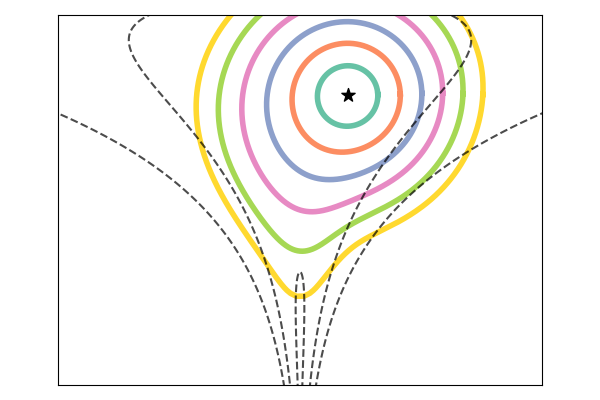
\includegraphics[width=\linewidth]{figs/paper2/geodesic_balls_generative.png}
        \caption{Generative metric.}
    \end{subfigure}
    \begin{subfigure}[b]{0.4\linewidth}
        \centering
        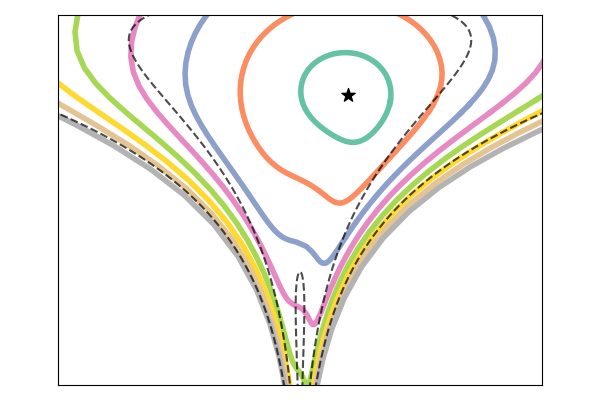
\includegraphics[width=\linewidth]{figs/paper2/geodesic_balls_monge.png}
        \caption{Monge metric.}
    \end{subfigure}
    \begin{subfigure}[b]{0.4\linewidth}
        \centering
        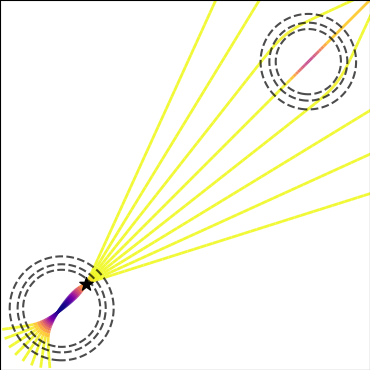
\includegraphics[width=0.8\linewidth]{figs/paper2/geodesic_inverse_generative.png}
        \caption{Inverse generative metric.}
    \end{subfigure}    
    \begin{subfigure}[b]{0.4\linewidth}
        \centering
        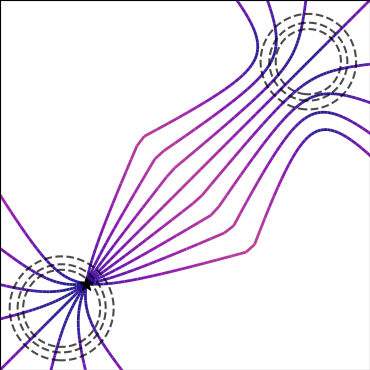
\includegraphics[width=0.8\linewidth]{figs/paper2/geodesic_inverse_monge.png}
        \caption{Inverse Monge metric.}
    \end{subfigure}    
    \caption{Visualization of the generative, inverse generative, Monge and inverse Monge metrics. \textbf{Top:} geodesic balls of varying radii centered at $\star$. \textbf{Bottom:} geodesics originating at $\star$ with different initial velocities (yellow indicates higher speed). The Monge metric deviates more from the Euclidean geometry than the generative metric, while the generative metric accelerates more in low-density regions.
   }
    \label{fig:metric_visualization}
\end{figure}
\begin{equation*}
    \mathbf{G}(\boldsymbol{x}) = \rho(\boldsymbol{x})^2 \mathbf{I}_D,
    \qquad
    \rho(\boldsymbol{x}) := \frac{p_0 + \lambda}{p(\boldsymbol{x}) + \lambda},
\end{equation*}
where $p_0, \lambda>0$ prevent the metric from becoming singular when $p(\boldsymbol{x})$ is small.
Since this metric is the identity matrix scaled, the inverse and determinant are straight to compute. The Christoffel symbols depend only on the gradient of the scalar factor,
\begin{equation*}
\Gamma^k(\boldsymbol{x}) = \nabla \log \rho(\boldsymbol{x}) \,\boldsymbol{e}_k^\top
+ \boldsymbol{e}_k \,\nabla \log \rho(\boldsymbol{x})^\top
- \partial_k \log \rho(\boldsymbol{x}) \,\mathbf{I}_D.
\end{equation*}

\begin{observation}[High-density regions are cheaper under the generative metric] \label{obs:generative}
Let
\begin{equation*}
\mathbf G(\boldsymbol x)=\rho(\boldsymbol x)^2 \mathbf I_D,
\qquad
\rho(\boldsymbol x)=\frac{p_0+\lambda}{p(\boldsymbol x)+\lambda},
\qquad p_0,\lambda>0.    
\end{equation*}
Then the Riemannian length of a piecewise \(C^1\) curve \(\gamma:[0,1]\to\mathbb R^D\) is
\begin{equation*}
L_{\mathbf G}(\gamma)=
\int_0^1
\|\dot \gamma(t)\|_{\mathbf G(\gamma(t))} \,
d t
=
\int_0^1 \left(\frac{p_0+\lambda}{p(\boldsymbol x)+\lambda}\right) \|\dot\gamma(t)\|_2\,dt.    
\end{equation*}
This weighted average results in geodesics that have a tradeoff between higher density values and shorter velocity Euclidean norms.
\end{observation}


\paragraph{The inverse metrics}
We have now introduced the Fisher, Monge and generative metrics. Now, we propose using the inverse metric to sample multimodal distributions. In general, any Riemannian tensor that is positive definite and full rank is mathematically valid. In particular, the inverse of the metrics is also positive definite and defines a valid metric tensor. This motivates defining the inverse metric
\begin{equation}
\boxed{
    \mathbf{G}_{\mathrm{inv}}(\boldsymbol{x}) = \mathbf{G}^{-1}(\boldsymbol{x}).
}
\end{equation}
The determinant is $\det \mathbf{G}_{\mathrm{inv}}(\boldsymbol{x})  = 1/\det \mathbf{G}(\boldsymbol{x})$. The Christoffel symbols are analytic and computable with automatic differentiation for the Monge and generative metrics. 

By Observations~\ref{obs:monge} and~\ref{obs:generative} the Monge and generative metrics induce geodesics that tend to stay within regions of high density. By using the inverse metric we hope to ``revert'' this property. In regions of low density, both the generative and Monge metrics assign larger Euclidean metric values, so their inverses effectively ``speed up'' motion.
As a result, geodesics can cover larger Euclidean distances over the same amount of geodesic time. This behavior is formalized in Observations~{\ref{obs:invmonge}} and~{\ref{obs:invgen}}. Figure~\ref{fig:metric_visualization} illustrates the properties of the inverse generative and inverse Monge metrics on a bimodal distribution. Although this does not guarantee that a geodesic will move from one mode to another in dimensions $D\geq 2$, we empirically observe in Section~\ref{sec:geodesic_slice} that the geodesics under the inverse Monge metric are capable of traversing between modes of multimodal distributions. 

\begin{observation}[Paper II]
\emph{
    Let $p(\boldsymbol{x})$ be a smooth density function. Let $(\boldsymbol{x}_t, \boldsymbol{v}_t)$ be the geodesic flow with initial conditions $(\boldsymbol{x}_0,\boldsymbol{v}_0)$  with respect to the inverse Monge metric, such that $\boldsymbol{x}_0$ is a local maximum.
    Then $\norm{\boldsymbol{v}_t}_{2}\geq \norm{\boldsymbol{v}_0}_{2}$ 
    for all $t\neq 0$.
    } \label{obs:invmonge}
\end{observation}
\begin{observation}[Paper II]
\emph{
    Let $p(\boldsymbol{x})$ be a smooth density function. Let $(\boldsymbol{x}_t, \boldsymbol{v}_t)$ be the geodesic flow with initial conditions $(\boldsymbol{x}_0,\boldsymbol{v}_0)$ such that $p(\boldsymbol{x}_0)>0$ with respect to the inverse generative metric. Then, for $t$ such that $p(\boldsymbol{x}_t) \to 0$ we have $\norm{\boldsymbol{v}_t}_{2}>\norm{\boldsymbol{v}_0}_{2}$.
    } \label{obs:invgen}
\end{observation}


 
\subsection{Volume form and density on the manifold}

\paragraph{Geodesic balls}
In both methods considered later,  we need to sample tangent vectors at a unit geodesic distance of a fixed point. 
For $\boldsymbol{x}\in\mathbb{R}^D$ the tangent space sphere of radius $r$ is
\begin{equation*}
\mathbb{S}^{D-1}_{\mathbf{G},r}(\boldsymbol{x})
:=
\left\{
\boldsymbol{v}\in T_{\boldsymbol{x}}\mathbb{R}^D :
\|\boldsymbol{v}\|_{\mathbf{G}(\boldsymbol{x})}= r
\right\}.
\end{equation*}
In practice we need to sample uniformly from the tangent space unit sphere which can be done as follows:
\begin{enumerate}
    \item Sample $\boldsymbol{v} \sim \mathcal{N}(\boldsymbol{0}, \mathbf{G}^{-1}(\boldsymbol{x}))$.
    \item Normalize $\boldsymbol{v} \leftarrow {\boldsymbol{v}}/{\|\boldsymbol{v}\|_{\mathbf{G}(\boldsymbol{x})}}$.
\end{enumerate}
Note that sampling $\boldsymbol{v} \sim \mathcal{N}(\boldsymbol{0}, \mathbf{G}^{-1}(\boldsymbol{x}))$ requires computing the inverse square root matrix $\mathbf{G}^{-1/2}$ which requires generally Cholesky decomposition, but for the Monge, generative, inverse Monge and inverse generative metrics it admits an analytic form. 

\paragraph{Hausdorff density}
The original target density $p(\boldsymbol{x})$ is defined with respect to Lebesgue measure in $\mathbb{R}^D$. Once a Riemannian metric is introduced, the natural reference measure becomes the Riemannian volume element \citep{Lee2018}, which is
\begin{equation*}
    d\mathrm{vol}_{\mathbf{G}}(\boldsymbol{x}) = \sqrt{\det \mathbf{G}(\boldsymbol{x})}\,d\boldsymbol{x}.
\end{equation*}
If we want to represent the density with respect to the volume element instead of Lebesgue measure, it must be rescaled by the corresponding factor.  We refer to this density as the Hausdorff density and write
\begin{equation} 
  p_{\mathcal{H}}(\boldsymbol{x}) := \frac{p(\boldsymbol{x})}{\sqrt{\det \mathbf{G}(\boldsymbol{x})}}. \label{eq:hausdensity}
\end{equation}
This is consistent with change of variables formula. Consider the  diffeomorphism  $\boldsymbol{z} = \varphi(\boldsymbol{x})$, change of variables gives
\begin{equation*}
    p_{\mathcal{Z}}(\boldsymbol{z}) = p(\varphi^{-1}(\boldsymbol{z})) \left|\det \mathbf{J}_{\varphi^{-1}}(\boldsymbol{x})\right|.
\end{equation*}
If $\mathbf{G}$ is the push-forward of the Euclidean metric under $\varphi$, then $\mathbf{G}(\boldsymbol{z})  = \mathbf{J}_{\varphi^{-1}}(\boldsymbol{z})^\top
    \mathbf{J}_{\varphi^{-1}}(\boldsymbol{z})$, and hence $\sqrt{\det \mathbf{G}(\boldsymbol{z})} = \left|\det \mathbf{J}_{\varphi^{-1}}(\boldsymbol{z})\right|$, and the change of variables formula can be written as
\begin{equation*}
    p_{\mathcal{Z}}(\boldsymbol{z}) = p(\varphi^{-1}(\boldsymbol{z}))  \sqrt{\det \mathbf{G}(\boldsymbol{z})}.
\end{equation*}
The density with respect to the Riemannian volume measure is
\begin{equation*}
    p_{\mathcal H}(\boldsymbol{z})
    =
    \frac{p_{\mathcal{Z}}(\boldsymbol{z})}{\sqrt{\det \mathbf{G}(\boldsymbol{z})}}. 
\end{equation*}
That is, the Hausdorff density removes the Jacobian volume factor and gets the density expressed with respect to the geometry induced by the metric.



\subsection{Numerical computation of geodesics}
For the Euclidean metric we can easily compute the exponential and logarithmic maps as in Equation~\ref{eq:Euclidean_exp_log}, but for the other metric choices we solve the geodesic equations numerically. Let $\boldsymbol{x}(t)$ denote the geodesic trajectory and $\boldsymbol{v}(t)=\boldsymbol{\dot x}(t)$ its velocity. Equation~\ref{eq:geodesic_equations} is rewritten as
\begin{align}
      \boldsymbol{ \dot x}(t)  &= \boldsymbol{v}(t), \nonumber \\
    \dot v_k(t) &= - \boldsymbol{v}(t)^\top\Gamma^k(\boldsymbol{x}(t))  \boldsymbol{v}(t), \quad  k = 1, \ldots, D, \label{eq:geoeqs}
\end{align}
where $\Gamma^k(\boldsymbol{x})\in\mathbb{R}^{D\times D}$ is the matrix with the Christoffel symbols (Equation~\ref{eq:christoffel_symbols}). 
The main computational bottleneck comes from the Christoffel symbols, since they involve the inverse metric and derivatives of the metric. The Fisher metric in general has $\mathcal{O}(D^3)$ complexity, the Monge and inverse Monge metrics have the complexity of Hessian-vector products, and the generative and inverse generative metrics have the complexity of gradient computations.

The choice of numerical solver affects accuracy and runtime \citep{kidger2022neural}. Fixed step-size, adaptive and higher order solvers introduce tradeoffs between stability, numerical error and computational cost. We conduct empirical studies on the choice of numerical solver for different metric choices in Section~\ref{sec:geodesic_slice}.



\begin{table}[t]
\centering
\footnotesize
\setlength{\tabcolsep}{4pt}
\begin{adjustbox}{max width=\linewidth}
\begin{tabular}{@{}lccc@{}}
\toprule
 & \textbf{Funnel} & \textbf{Rosenbrock} & \textbf{Squiggle} \\
\midrule
$\varphi(\boldsymbol{z})$
&
$\left[
\begin{array}{c}
e^{\sigma z_D /2} \boldsymbol{z}_{1:D-1}\\
\sigma z_D
\end{array}
\right]$
&
$\left[
\begin{array}{c}
a + \tfrac{1}{\sqrt{2}}z_1 \\
\left(a + \tfrac{1}{\sqrt{2}}z_1\right)^2 + \tfrac{1}{\sqrt{2b}}z_2
\end{array}
\right]$
&
$\left[
\begin{array}{c}
z_1 \\
\boldsymbol{z}_{2:D} - \sin(a z_1)
\end{array}
\right]$
\\
\midrule
$p(\boldsymbol{x})$
&
$\begin{aligned}
&\mathcal{N}(x_D \mid 0,\sigma^2)\\
&\times\mathcal{N}(\boldsymbol{x}_{1:D-1} \mid \boldsymbol{0}, e^{x_D}\mathbf{I}_{D-1})
\end{aligned}$
&
$\begin{aligned}
&\mathcal{N}(x_1 \mid a, \tfrac{1}{2})\\
&\times\mathcal{N}(x_2 \mid x_1^2, \tfrac{1}{2b})
\end{aligned}$
&
$\begin{aligned}
&\mathcal{N}\!\bigl(\varphi^{-1}(\boldsymbol{x}) \mid \boldsymbol{\mu}, \mathbf{\Sigma}\bigr)\\
&\times\left|\det \mathbf{J}_{\varphi^{-1}}(\boldsymbol{x})\right|
\end{aligned}$
\\
\midrule
&
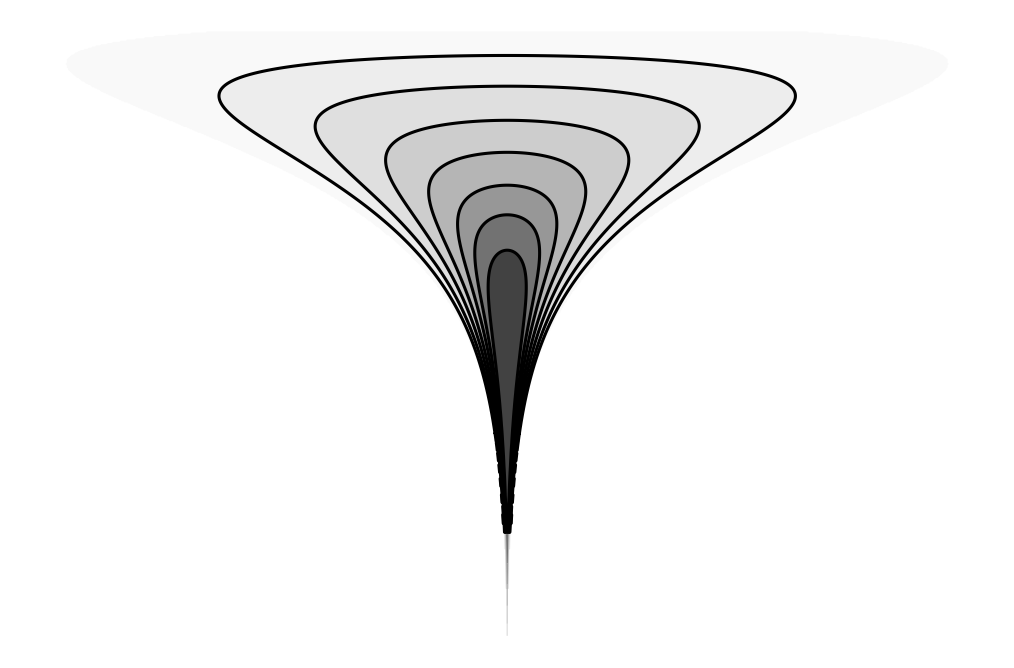
\includegraphics[width=0.32\linewidth]{figs/extra/funnel_contour.png}
&
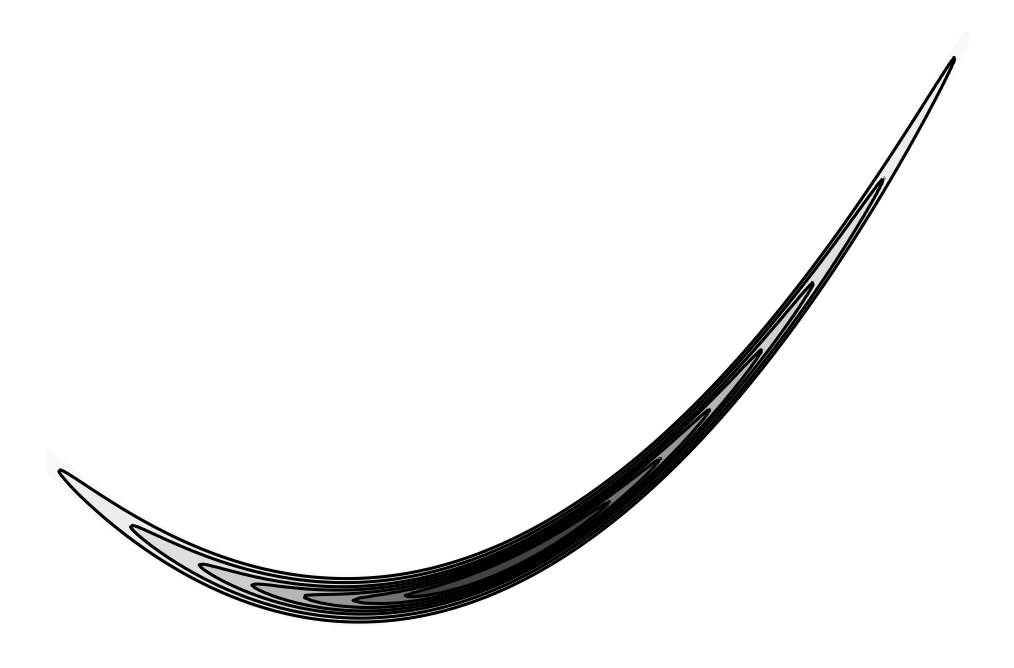
\includegraphics[width=0.32\linewidth]{figs/extra/rosenbrock_contour.png}
&
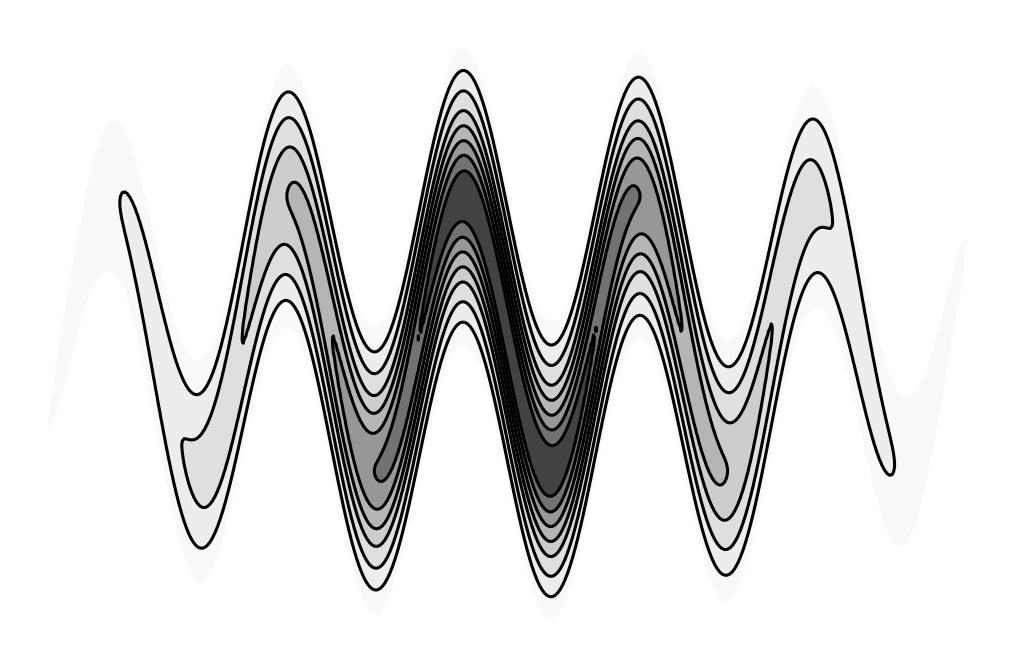
\includegraphics[width=0.32\linewidth]{figs/extra/squiggle_contour.png} \\
% \bottomrule 
\end{tabular}
\end{adjustbox}
\caption{Three benchmark distributions with strong curvature used in the experiments.}
\label{tab:curved_distributions}
\end{table}

\subsection{Target distributions with strong curvature} \label{sec:curved}
The need for a non-Euclidean metric is most pronounced in regions of the parameter space that are narrow along certain directions but still carry significant probability mass. For evaluation of these methods we hence consider three distributions with strong curvature that are constructed from a diffeomorphism of a standard Gaussian. They are the Funnel, Hybrid Rosenbrock and Squiggle distributions. Here we present a simpler version of the Hybrid Rosenbrock, the $D$-dimensional version is given in \citet{Pagani2022}. Table~\ref{tab:curved_distributions} shows the distributions, summarizes the transformations and the corresponding target densities.

The latent value is distributed  $\boldsymbol{z}\sim \mathcal{N}(\boldsymbol{\mu},\mathbf{\Sigma})$ and $\boldsymbol{x}=\varphi(\boldsymbol{z})$.
The bijection $\varphi$ allows the generation of samples for benchmarking. The pullback metric follows from the transformation rule of Riemannian tensors,
\begin{equation}
\mathbf{G}(\boldsymbol{x})
=
\mathbf{J}_{\varphi^{-1}}(\boldsymbol{x})^\top
\mathbf{\Sigma}^{-1}
\mathbf{J}_{\varphi^{-1}}(\boldsymbol{x}).
\label{eq:pullback_metric_curved}
\end{equation}

\section{Case study I: Riemannian Laplace approximation} \label{sec:rla}

We apply the geometric tools we have described above in the construction of Riemannian Laplace approximation (RLA) \citep{Bergamin2024}. We first use a second order Taylor approximation to motivate placing a Gaussian distribution in the tangent space at the mode. Sampling is then done by drawing Gaussian velocities in this tangent space, and pushing them forward with the exponential map. RLA can be viewed as an exponential wrapped Gaussian approximation where the geometry is determined by the chosen metric tensor (see Figure~\ref{fig:rla}).
\begin{figure}
    \centering
    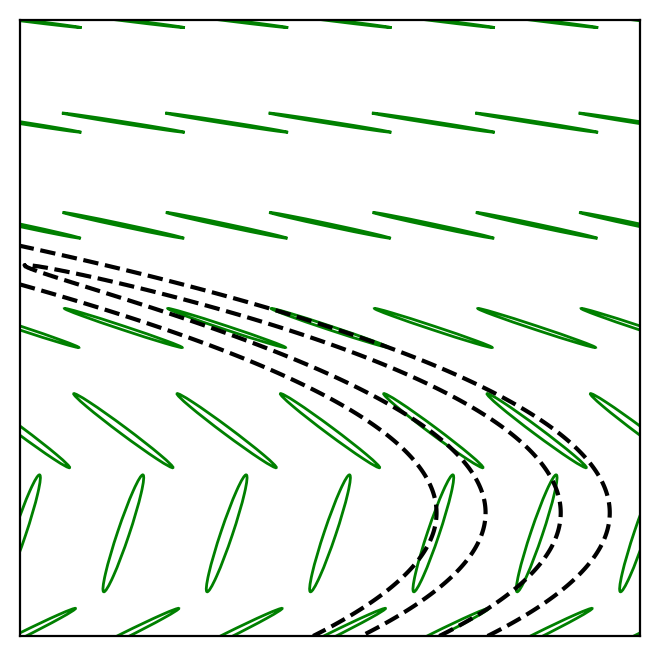
\includegraphics[width=0.3\linewidth]{figs/paper1/metrics.png}
    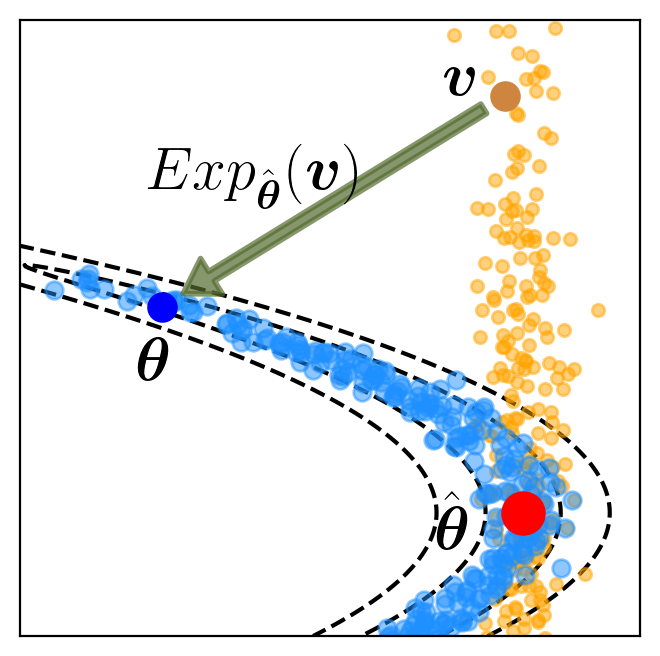
\includegraphics[width=0.3\linewidth]{figs/paper1/geodesics.png}
    \caption{Visualization of Riemannian Laplace approximation. The Fisher metric (green) captures the local curvature. Right: Samples from a Gaussian distribution (orange) are deterministically mapped using the Fisher metric to provide a flexible approximation (blue).}
    \label{fig:rla}
\end{figure}

Let $f$ be a scalar output function defined on the manifold and $c(t)$ a curve on the manifold such that $c(0)= \boldsymbol{x}$. As given in Section~5.9, Equation~5.26, of \citet{Boumal2023}, the second-order Taylor approximation is
\begin{equation} \label{eq:taylor_mfd}
    \begin{aligned}
    f(c(t)) = f(\boldsymbol{x})
&+ t \left\langle \nabla_{\mathbf{G}} f(\boldsymbol{x}), \boldsymbol{v} \right\rangle_{\mathbf{G}(\boldsymbol{x})}
+ \frac{t^2}{2} \left\langle \operatorname{Hess}_{\mathbf{G}} f(\boldsymbol{x})[\boldsymbol{v}], \boldsymbol{v} \right\rangle_{\mathbf{G}(\boldsymbol{x})} \\
&+ \frac{t^2}{2} \left\langle \nabla_{\mathbf{G}} f(\boldsymbol{x}), \ddot{c}(0) \right\rangle_{\mathbf{G}(\boldsymbol{x})}
+ \mathcal{O}(t^3).        
    \end{aligned}
\end{equation}
Let $\ell$ be the target logdensity (Euclidean or Hausdorff) and $\hat{\boldsymbol{x}}$ a local maximum of $\ell$. 
At the mode $\hat{\boldsymbol{x}}$, both Euclidean and Riemannian gradients vanish, and a second order Taylor expansion of $\ell$ along geodesics (Equation~\ref{eq:taylor_mfd})  simplifies to
\begin{equation}\label{eq:riemlap}
\ell\big(\operatorname{Exp}_{\hat{\boldsymbol{x}}}(\boldsymbol{v})\big)
\approx \ell(\hat{\boldsymbol{x}})
+ \tfrac{1}{2}\, 
\left\langle
\operatorname{Hess}_{\mathbf{G}}\,\ell(\hat{\boldsymbol{x}})[\boldsymbol{v}],
\boldsymbol{v}
\right\rangle_{\mathbf{G}(\boldsymbol{\hat{x}})},
\end{equation}
where $t$ is absorbed into $\boldsymbol{v}\gets t \boldsymbol{v}$. 
Furthermore, the Riemannian Hessian components (Equation~\ref{eq:riem_hessian}) simplify to
\begin{equation*}
 \mathrm{Hess}_{\mathbf{G}} \ell(\boldsymbol{\hat{x}}) [\boldsymbol{v}] = \mathbf{G}^{-1}(\boldsymbol{\hat{x}})\nabla^2\ell ({\boldsymbol{\hat{x}}}) \boldsymbol{v},
\end{equation*}
since $\nabla \ell(\hat{\boldsymbol{x}}) = \boldsymbol{0}$ \footnote{personal communication with Marcelo Hartmann}.
Thus, the quadratic term in Equation~\ref{eq:riemlap} is 
$\boldsymbol{v}^{\top}\nabla^2\ell(\hat{\boldsymbol{x}})\boldsymbol{v}$
, which motivates a tangent space Gaussian density
\begin{equation*}
 h_{\mathbf{\Sigma}}(\boldsymbol{v})=\mathcal{N}(\boldsymbol{v}\mid\boldsymbol{0}, \mathbf\Sigma), \quad   \mathbf\Sigma = \left(-\nabla^2\ell(\hat{\boldsymbol{x}})\right)^{-1}. 
\end{equation*} 
Samples that approximate the target are generated by mapping the exponential map on the tangent velocities (see Algorithm~\ref{alg:rla}), this is the core principle of the method
\begin{equation}
\boxed{
    \boldsymbol{x}=\operatorname{Exp}_{\hat{\boldsymbol{x}}}(\boldsymbol{v}), \quad \boldsymbol{v}\sim \mathcal{N}(\boldsymbol{0}, \mathbf\Sigma).
    }
\end{equation}
We can compute the RLA logdensity associated to the samples in the tangent space radius where the exponential map is injective  \citep{chevallier2022exponential}.
The push-forward density of the tangent Gaussian
with respect to the Riemannian volume is given by the exponential-wrapped change of variables
\begin{equation*}
\log q_{\mathcal H}(\boldsymbol{x})
=
\log h_{\mathbf{\Sigma}}(\boldsymbol{v})
-
\log \left|\det J_{\hat{\boldsymbol{x}}}(\boldsymbol{v}) \right|,
\end{equation*}
where $\boldsymbol{x}=\operatorname{Exp}_{\hat{\boldsymbol{x}}}(\boldsymbol{v})$ and  $\mathbf{J}_{\hat{\boldsymbol{x}}}(\boldsymbol{v})= \mathrm{d}_{\boldsymbol{v}}
\operatorname{Exp}_{\hat{\boldsymbol{x}}}(\boldsymbol{v})$. In general RLA settings the differential of the exponential map may need to be computed numerically. On affine locally symmetric spaces, however, it admits an explicit curvature-based series expansion, which yields tractable Jacobian formulas \citep{chevallier2022exponential}.
 

\begin{algorithm}[t]
	    \caption{RLA, producing $N$ samples $\boldsymbol{x}^{(n)}$.}    
	    \begin{algorithmic}[1]        
	    \Require Metric $\mathbf{G}$ and covariance $\mathbf{\Sigma}$
	        \State Obtain the MAP estimate $\hat{\boldsymbol{x}}$.        
	        \For{$n \leftarrow 1\dots N$}            
	            \State Obtain $\boldsymbol{v}^{(n)}\sim \mathcal{N}(\boldsymbol{0}, \mathbf{\Sigma})$
	            \State Push-forward $\boldsymbol{x}^{(n)} \gets \operatorname{Exp}_{\hat{\boldsymbol{x}}}(\boldsymbol{v}^{(n)})$
	        \EndFor
	\end{algorithmic}
	\label{alg:rla}
\end{algorithm}

\citet{Bergamin2024} proposed using the Monge metric in the RLA approximation, which we denote RLA-B. Although the Monge metric has lower complexity than Fisher metric, this approximation is biased for Gaussian targets as a consequence of  Observation~\ref{obs:monge}. The Monge geodesics contract Euclidean distances near a mode and samples generated by the geodesics under this metric are too close to the mode, while the Euclidean Laplace is exact. 

Paper I proposes two improvements that correct this behavior:
\begin{itemize}
    \item Apply a logarithm map to correct the magnitude of the velocities. Namely, replace Step~3 in Algorithm~\ref{alg:rla} with 
    \begin{align*}
	\tilde{\boldsymbol{x}}^{(n)} &\sim \mathcal{N}\!\left(\hat{\boldsymbol{x}}, (-\nabla^2 \ell(\hat{\boldsymbol{x}}))^{-1}\right), \text{ and} \\
	\boldsymbol{v}^{(n)} &= \operatorname{Log}_{\mathcal{P},\hat{\boldsymbol{x}}}(\tilde{\boldsymbol{x}}^{(n)}),
	\end{align*}    
    where $\operatorname{Log}_{\mathcal{P},\hat{\boldsymbol{x}}}$ is computed with respect to the Monge metric induced by the density $\mathcal{N}\!\left(\hat{\boldsymbol{x}}, (-\nabla^2 \ell(\hat{\boldsymbol{x}}))^{-1}\right)$, we refer to this variant as RLA-BLog.
    \item Use the Fisher information metric in Riemannian Laplace approximation, denoted RLA-F.
\end{itemize}

Additionally, Paper~I studies practical choices: whether the approximation should be centered at the Euclidean MAP or at the Hausdorff MAP and whether $\mathbf{\Sigma}=(-\nabla^2\ell(\boldsymbol{\hat{x}}))^{-1}$ or $\mathbf{\Sigma}=\mathbf{G}^{-1}(\boldsymbol{\hat{x}})$ should be used.
Paper~I also provides theoretical advantages for the Fisher metric. It is exact for Gaussian targets, asymptotically for targets that are Gaussian in the limit of infinite data, and it is  exact for targets that are diffeomorphic to a Gaussian. Theorem~\ref{thm:invariant-exact} states the exactness of RLA-F for Gaussian diffeomorphism. 

\begin{theorem}[\textbf{Paper I - Theorem 3}]
    With an invariant prior, e.g. Jeffreys prior, 
    RLA-F with Hausdorff MAP is exact for probabilistic models whose target distributions are diffeomorphic with Gaussians, for which the negative Hessian at the Hausdorff MAP coincides with the Fisher metric.
\label{thm:invariant-exact}
\end{theorem}


\subsection*{Empirical evaluation}
The empirical study compares Euclidean Laplace approximation (ELA), the Monge-based approximation (RLA-B), the logarithm-map corrected Monge variant (RLA-BLog), and the Fisher variant (RLA-F).
Here we include two of the experiments from Paper~I, the objective of the first experiment is to visually illustrate each of the methods and the effect of the Hausdorff MAP. The second experiment shows that even though RLA-F is more expensive than Monge due to the cubic complexity, it can be more efficient in the number of steps needed by an adaptive numerical integrator which makes the RLA-F the recommended choice for problems where the Fisher is computable and with tens to low hundreds of dimensions. Since all Riemannian variants require solving geodesic equations numerically, in all experiments we use the same Dopri5 adaptive integrator \citep{kidger2022neural}.

\paragraph{Visual illustration of Riemannian Laplace}
The first experiment is a visual comparison on the Banana distribution. Figure~\ref{fig:banana} shows the approximations obtained from both the Euclidean target density (first column) and the corresponding Hausdorff density (second column).
The takeaway message is that Euclidean Laplace approximation does not capture the curvature, and among the geometry-aware methods the Fisher information produces the best fit to the target distribution, note how RLA-B samples do not properly spread out  without the Log-corrector.

\begin{figure}
    \centering    
    \begin{tabular}{@{}rcc@{}} 
        & Euclidean MAP & Hausdorff MAP \\
        ELA &
        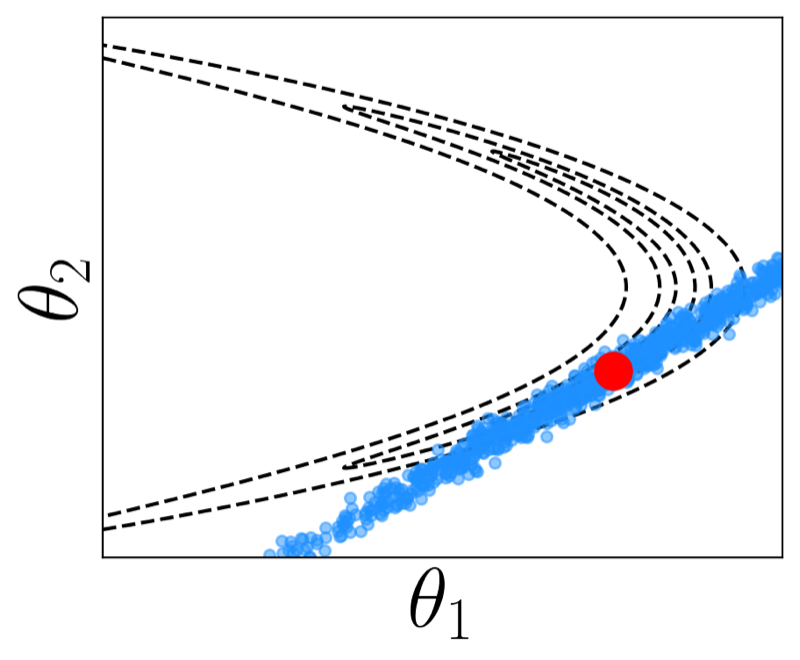
\includegraphics[width=0.38\textwidth, valign=m]{figs/paper1/h_banana_euclidean.png} & 
        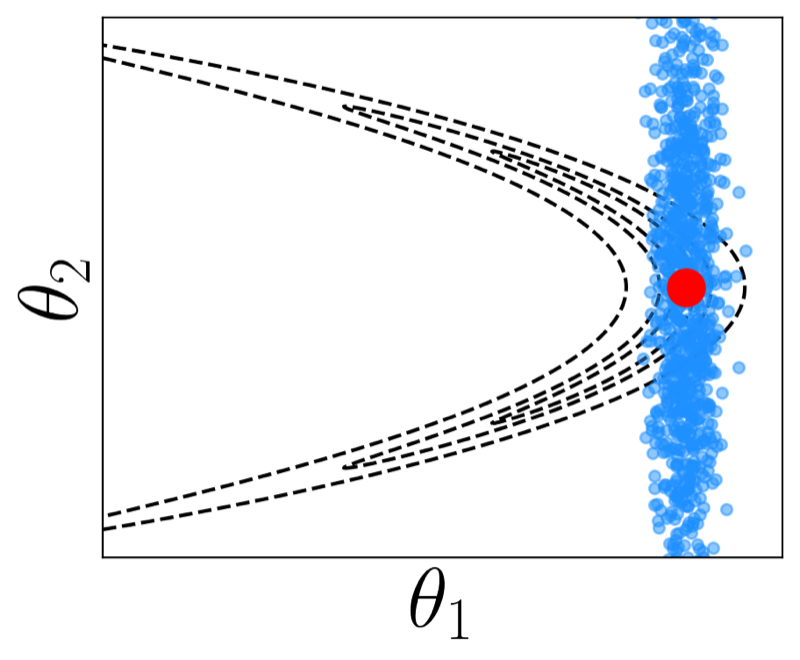
\includegraphics[width=0.38\textwidth, valign=m]{figs/paper1/f_banana_hausdorff_euclidean.png} \\
        RLA-B &
        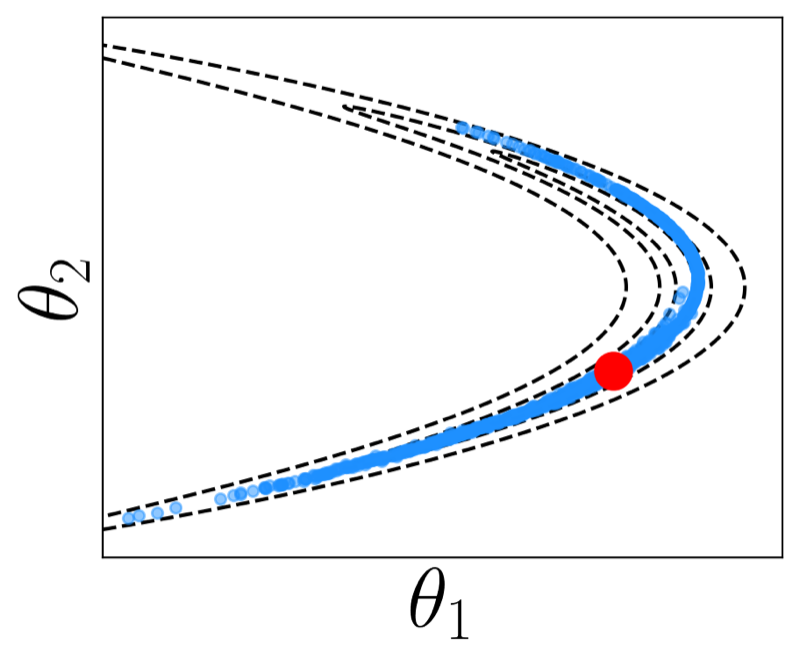
\includegraphics[width=0.38\textwidth, valign=m]{figs/paper1/h_banana_bergamin.png} & 
        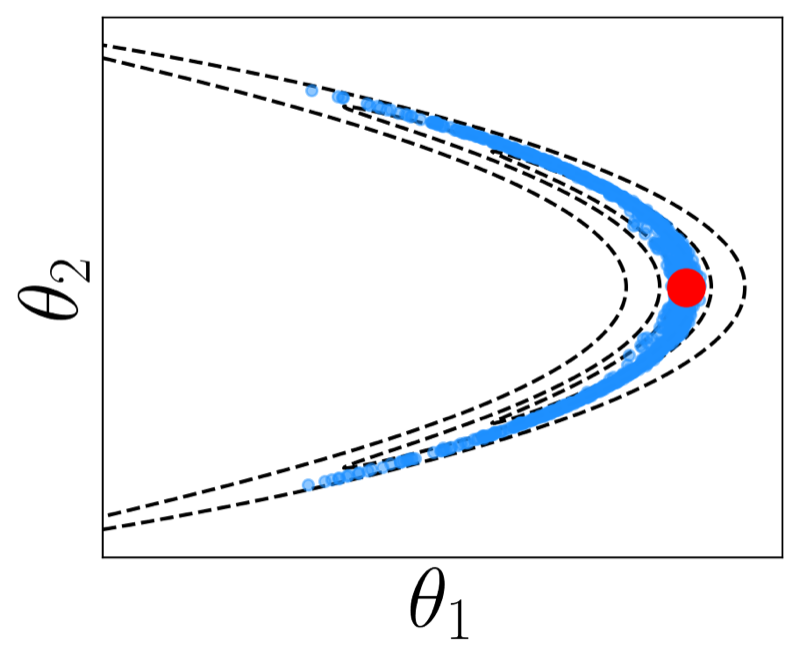
\includegraphics[width=0.38\textwidth, valign=m]{figs/paper1/f_banana_hausdorff_bergamin.png} \\
        RLA-BLog &
        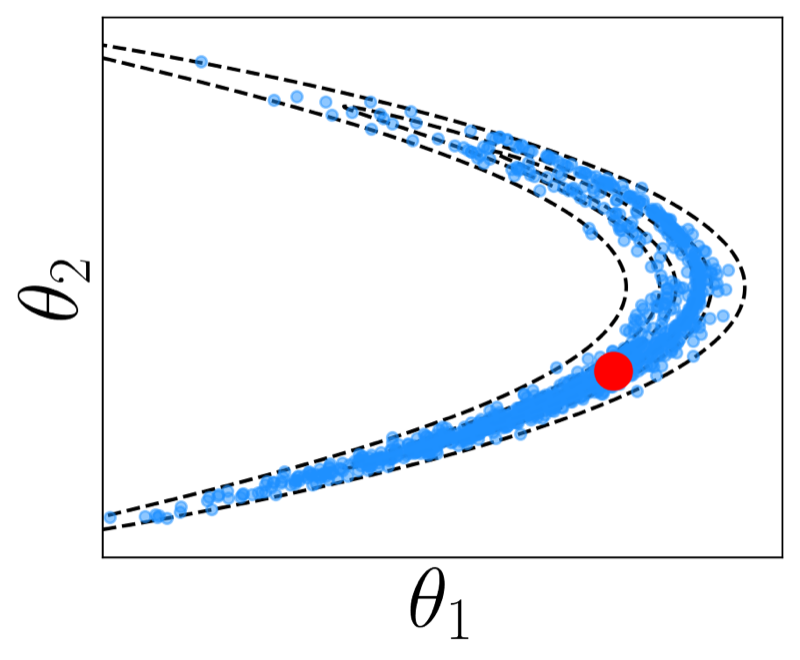
\includegraphics[width=0.38\textwidth, valign=m]{figs/paper1/h_banana_monge.png} & 
        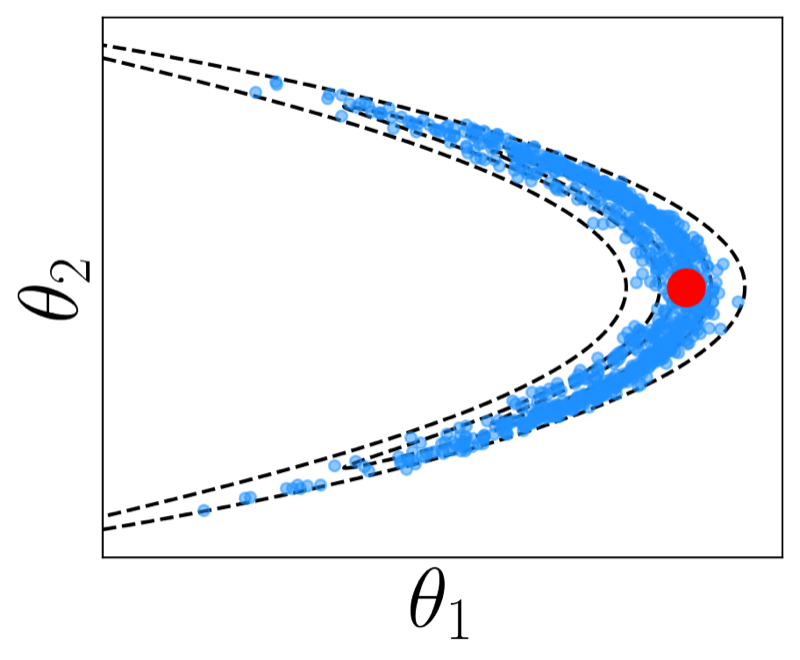
\includegraphics[width=0.38\textwidth, valign=m]{figs/paper1/f_banana_hausdorff_monge.png} \\
        RLA-F &
        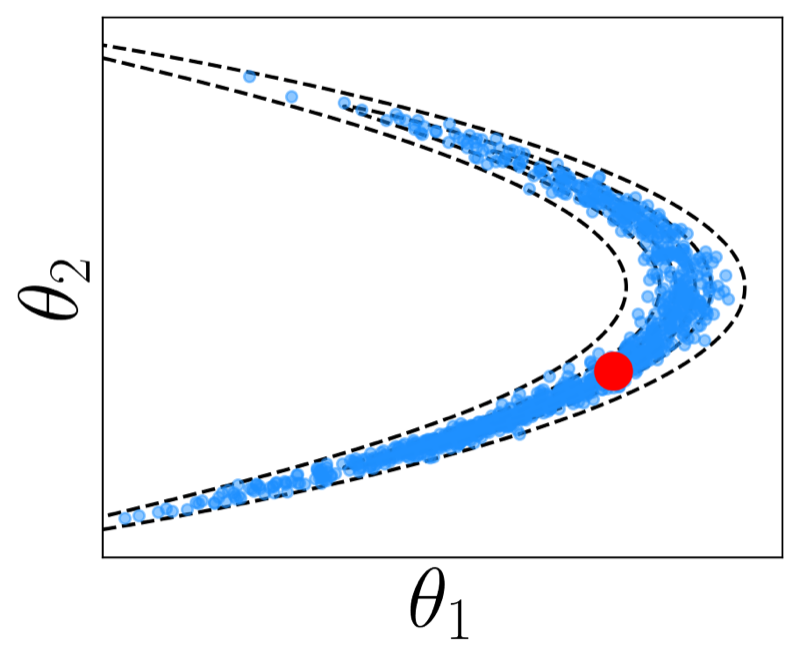
\includegraphics[width=0.38\textwidth, valign=m]{figs/paper1/h_banana_fisher.png} & 
        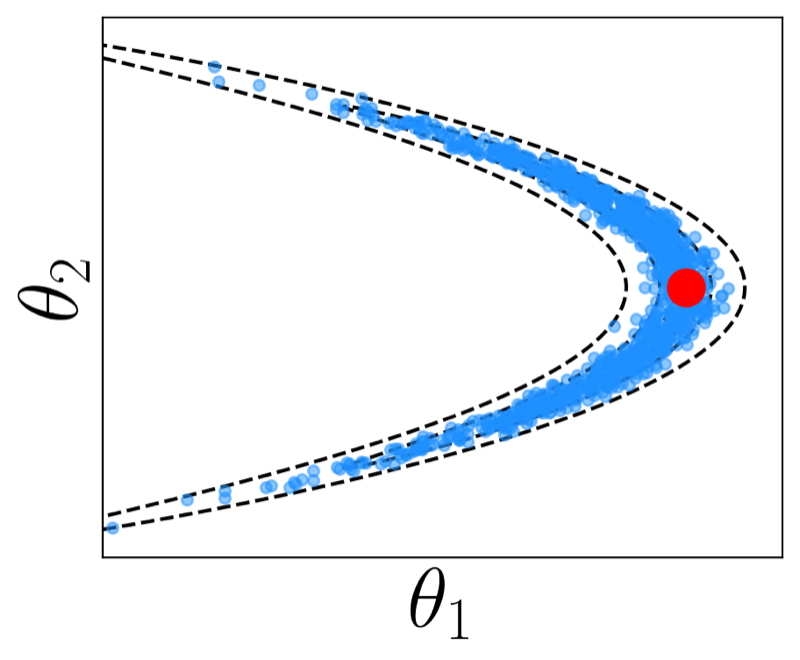
\includegraphics[width=0.38\textwidth, valign=m]{figs/paper1/f_banana_hausdorff_fisher.png}         
    \end{tabular}
    \caption{Comparison of Euclidean and Hausdorff MAP estimates. The red points are the Euclidean or Hausdorff MAP, and samples are scatter points in blue. The Euclidean metric (ELA) does not capture the geometry. The Monge metric is narrow without the logarithm map adjustment (RLA-B). The Fisher metric(RLA-F) is the most accurate with Hausdorff MAP. }
    \label{fig:banana}
\end{figure}


\paragraph{Efficiency of the approximation}
The second experiment considers Bayesian logistic regression on several benchmark data sets, both with standardized inputs and with raw inputs. The Fisher metric includes the Hessian of the prior as in Equation~\ref{eq:fisher_w_prior}. Table~\ref{tbl:lr} reports the Wasserstein distance to reference samples obtained with NUTS and the average number of log-density evaluations per sample.  The main takeaway is that 
RLA-F is more efficient in integration steps (geodesics are easier to integrate) and is more accurate than the Euclidean and Monge metric variants. 
\begin{table*}
	\centering
        \resizebox{\textwidth}{!}{
		\begin{tabular}{|l|l|l|l|l|l|l|l|l|}
			\hline
			 & & \multicolumn{1}{|c|}{ELA} & \multicolumn{2}{|c|}{RLA-B} & \multicolumn{2}{|c|}{RLA-BLog} & \multicolumn{2}{|c|}{RLA-F} \\
			\hline
			 & data & $\mathcal{W}$ & $\mathcal{W} \downarrow$ & $T$ & $\mathcal{W} \downarrow$ & $T$ & $\mathcal{W} \downarrow$ & $T$ \\
			\hline
			\multirow{5}{1em}{\centering\rotatebox[origin=c]{90}{stand.}}&Ripl & $0.106 \pm 0.004$ & $0.236 \pm 0.001$ & 29.7 & $0.16 \pm 0.065$ & 45.2 & $\textbf{0.064} \pm 0.002$ & \textbf{12.2} \\
			\cline{2-9}
			&Pima & $0.149 \pm 0.0$ & $0.274 \pm 0.0$ & 41.7 & $0.21 \pm 0.007$ & 78.5 & $\textbf{0.147} \pm 0.0$ & \textbf{12.2} \\
			\cline{2-9}
			&Hear & $0.529 \pm 0.001$ & $0.649 \pm 0.0$ & 40.2 & $1.154 \pm 0.189$ & 71.6 & $\textbf{0.514} \pm 0.0$ & \textbf{13.2} \\
			\cline{2-9}
			&Aust & $0.441 \pm 0.001$ & $0.522 \pm 0.001$ & 51.5 & $0.745 \pm 0.203$ & 79.1 & $\textbf{0.417} \pm 0.001$ & \textbf{18.0} \\
			\cline{2-9}
			&Germ & $0.388 \pm 0.001$ & $0.431 \pm 0.0$ & 58.4 & $0.676 \pm 0.1$ & 104.0 & $\textbf{0.387} \pm 0.0$ & \textbf{14.2} \\
			\hline
			\multirow{5}{1em}{\centering\rotatebox[origin=c]{90}{raw}}&Ripl & $0.437 \pm 0.017$ & $0.489 \pm 0.012$ & 30.2 & $0.554 \pm 0.253$ & 45.0 & $\textbf{0.247} \pm 0.012$ & \textbf{12.7} \\
			\cline{2-9}
			&Pima & $0.21 \pm 0.01$ & $0.294 \pm 0.004$ & 5632.9 & $0.216 \pm 0.014$ & 1690.4 & $\textbf{0.112} \pm 0.008$ & \textbf{15.4} \\
			\cline{2-9}
			&Hear & $0.842 \pm 0.026$ & $0.96 \pm 0.012$ & \textit{7868.2} & $0.898 \pm 0.029$ & \textit{3161.1} & $\textbf{0.644} \pm 0.012$ & \textbf{17.9} \\
			\cline{2-9}
			&Aust & $0.454 \pm 0.004$ & $0.455 \pm 0.01$ & \textit{18513.8} & $0.467 \pm 0.005$ & \textit{12298.6} & $\textbf{0.378} \pm 0.005$ & \textbf{18.0} \\
			\cline{2-9}
			&Germ & $0.846 \pm 0.002$ & $0.92 \pm 0.003$ & 3545.9 & $0.898 \pm 0.003$ & 2985.5 & $\textbf{0.823} \pm 0.001$ & \textbf{17.8} \\
			\hline
		\end{tabular}
        }	
	\caption{Logistic regression results as $\text{mean} \pm \text{std}$. Bold font indicates the best method. Italic font indicates the integrator reached maximum number of steps in at least one run. $\mathcal{W}$ indicates the 1-Wasserstein distance to NUTS samples while $T$ indicates the average number of function evaluations for one sample. For all evaluation metrics smaller is better.}
	\label{tbl:lr}
\end{table*}





\section{Case study II: geodesic slice sampling} \label{sec:geodesic_slice}
This case study uses the geometric tools from Section~\ref{sec:geometric_tools} in an MCMC sampling method.  In Section~\ref{sec:slice_sampling} we introduced  hit-and-run slice sampling that does slice sampling along Euclidean straight lines,  geodesic slice sampling from Paper~II keeps the same logic but replaces the straight lines by the geodesics induced by a metric choice. This change allows for MCMC sampling of distributions with strong curvature, multimodality or both.  

\paragraph{Geodesic slice sampling}
Our method builds on \citet{durmus2026geodesic}, who introduced geodesic slice sampling  over manifolds with closed form geodesics (e.g the sphere, torus, hyperbolic space,...). Paper~II extends this method to distributions defined on $\mathbb{R}^D$ with generic metric tensors $\mathbf{G}(\boldsymbol{x})$. Our method is metric-agnostic geodesic slice sampling (MAGSS).

In Euclidean hit-and-run slice sampling one first samples a random velocity $\boldsymbol{v}$ and performs univariate slice sampling on the straight line passing through the current state $\boldsymbol{x}$. Our method replaces the straight line 
$\boldsymbol{x} + t \boldsymbol{v}$ with the geodesic generated by the exponential map $\operatorname{Exp}_{\boldsymbol{x}}(t\boldsymbol{v})$, the target density $p(\boldsymbol{x})$ with the Hausdorff density $p_{\mathcal{H}}(\boldsymbol{x})$ and the Euclidean sphere $\mathbb{S}^{D-1}$ with the Riemannian sphere $\mathbb{S}^{D-1}_{\mathbf{G}}$  (see Table~\ref{tab:slice_compare}). Denote by  $\hat{\gamma}_{\boldsymbol{x},\boldsymbol{v}}(t)$ the numerical solution of the geodesic equations with initial conditions $\boldsymbol{x},\boldsymbol{v}$ for time $t$. Algorithm~\ref{alg:gss} shows the Geodesic Slice Sampling procedure.

\paragraph{Choice of metric}
Similar to Riemannian Laplace, the main modeling decision is the choice of Riemannian metric. For targets with strong local curvature, the Fisher, Monge and generative metrics can make geodesics better aligned with the shape of the density, with tradeoffs in the computational speed.

For multimodal targets, the inverse Monge and inverse generative metrics play a different role: they increase Euclidean speed in low-density regions and might be able to bridge between different modes, as discussed in Observations~\ref{obs:invmonge} and~\ref{obs:invgen}. In this sense, the same sampler can be adapted either to local geometry or to global mode exploration by changing only the metric tensor (as shown in Figure~\ref{fig:metric_visualization}). 
The Monge and generative metrics depend on hyperparameters. 
A limitation of our method is that there is no default value for these metric-parameters, some problems might allow for computation of a validation statistic for selection but no general value is optimal.


\paragraph{Meta-sampler} Paper II also considers a simple meta-sampler that alternates between geodesic slice sampling moves and local MCMC updates (e.g. MALA). The purpose of this combination is to use MAGSS with the inverse metrics for global transitions and the local Markov chain for exploration within each mode. This is particularly useful when the target is both multimodal and locally has high curvature. This is denoted by Meta-MAGSS. 



\begin{table}[t]
\centering
\small
\begin{tabular}{lll}
\toprule
 & Euclidean & Riemannian \\
\midrule
Slice level 
& $s \sim \mathrm{Unif}\!\bigl(0, p(\boldsymbol{x}^{(n)})\bigr)$
& $s \sim \mathrm{Unif}\!\bigl(0, \textcolor{mycolor}{p_{\mathcal{H}}}(\boldsymbol{x}^{(n)})\bigr)$ \\

Velocity 
& $\boldsymbol{v}^{(n)} \sim \mathrm{Unif}\!\bigl(\mathbb{S}^{D-1}(\boldsymbol{x}^{(n)})\bigr)$
& $\boldsymbol{v}^{(n)} \sim \mathrm{Unif}\!\bigl(\textcolor{mycolor}{\mathbb{S}^{D-1}_{\mathbf{G}}}(\boldsymbol{x}^{(n)})\bigr)$ \\

Slice sampling on 
& $\gamma_{\boldsymbol{x}^{(n)},\boldsymbol{v}^{(n)}}(t) = \boldsymbol{x}^{(n)} + t\boldsymbol{v}^{(n)}$
& $\textcolor{mycolor}{{\gamma}}_{\boldsymbol{x}^{(n)},\boldsymbol{v}^{(n)}}(t) 
= \textcolor{mycolor}{\operatorname{Exp}_{\boldsymbol{x}^{(n)}}}(t\boldsymbol{v}^{(n)})$ \\

\bottomrule
\end{tabular}
\caption{Comparison of Euclidean and Riemannian slice sampling components. Red highlights indicate the Riemannian modifications.}
\label{tab:slice_compare}
\end{table}



\begin{algorithm}[t]
    \caption{Geodesic slice sampling, producing $N$ samples $\boldsymbol{x}^{(n)}$.}    
	    \begin{algorithmic}[1]        
	    \Require Initial $\boldsymbol{x^{(0)}}$, metric $\mathbf{G}$ and parameters $m\in \mathbb{N}$, $w\ge 0$	        
	        \For{$n \leftarrow 0\dots N-1$}     
                \State Sample $s \sim \mathrm{Unif}(0, p_{\mathcal{H}}(\boldsymbol{x}^{(n)}))$ and $\boldsymbol{v}^{(n)} \sim \textrm{Unif}(\mathbb{S}_{\mathbf{G}}^{D-1}(\boldsymbol{x}^{(n)}))$
	            \State Obtain $(\ell, r) = \text{Step-out}_{w,m}(s, \hat{\gamma}_{\boldsymbol{x}^{(n)}, \boldsymbol{v}^{(n)}})$
	            \State Sample $t^* = \text{Shrink}_{\ell,r}(s, \hat{\gamma}_{\boldsymbol{x}^{(n)}, \boldsymbol{v}^{(n)}} )$
                \State Push-forward $\boldsymbol{x}^{(n+1)} \gets \hat{\gamma}_{\boldsymbol{x}^{(n)}, \boldsymbol{v}^{(n)}} (t^*)
                $
	        \EndFor
	\end{algorithmic}
	\label{alg:gss}
\end{algorithm}



\subsection*{Empirical evaluation}
The empirical evaluation compares parallel tempering (PT; \citealp{Latuszynski2025}), the diffusion Gibbs sampler (DiGS; \citealp{Chen2024}), and metric-agnostic geodesic slice sampling (MAGSS). We highlight some of the experiments from Paper~II. The objective of the experiments is to study our method on curved distributions and multimodal distributions, comparing the accuracy and running time against the alternatives. 

The first experiment shows MAGSS performance on curved target distributions. The second experiment compares the mode exploration of the methods on a highly multimodal target distribution modeling the Allen-Cahn field system. The third experiment studies the effect of the numerical integrator on our method. Paper~II gives the full description of the experimental setup and further analysis. 


\paragraph{Curved target distributions}
We consider the  Funnel, Rosenbrock and Squiggle target distributions with strong curvature from Section~\ref{sec:curved}. Figure~\ref{fig:toydistdims} shows the empirical 1-Wasserstein distance to reference samples from the distributions for dimensions $2,4,..2^8$. The Fisher metric produces the highest quality samples, but becomes computationally too expensive as can be seen by the cut-off in the lines, the Monge metric produces good results on Rosenbrock and Squiggle distributions. DiGS, PT and NUTS struggle exploring the curved regions of the space and are less accurate, note that DiGS uses the local MCMC  Metropolis-adjusted Langevin algorithm (MALA), a Riemannian version could be used instead to enhance exploration of the curved regions as an improvement to the method. The values of the hyperparameters of the Monge and generative metrics are $\alpha^2, \lambda=1$. 
We use the step-size value $w = 3$ and max iterations $m = 8$ in MAGSS.
DiGS uses a single noise scale of $1$ and NUTS and MALA (inside DiGS) use a stepsize of $0.1$. 

\begin{figure}[t]
    \centering
    \begin{minipage}{0.32\textwidth}
        \centering
        {Funnel}\\
        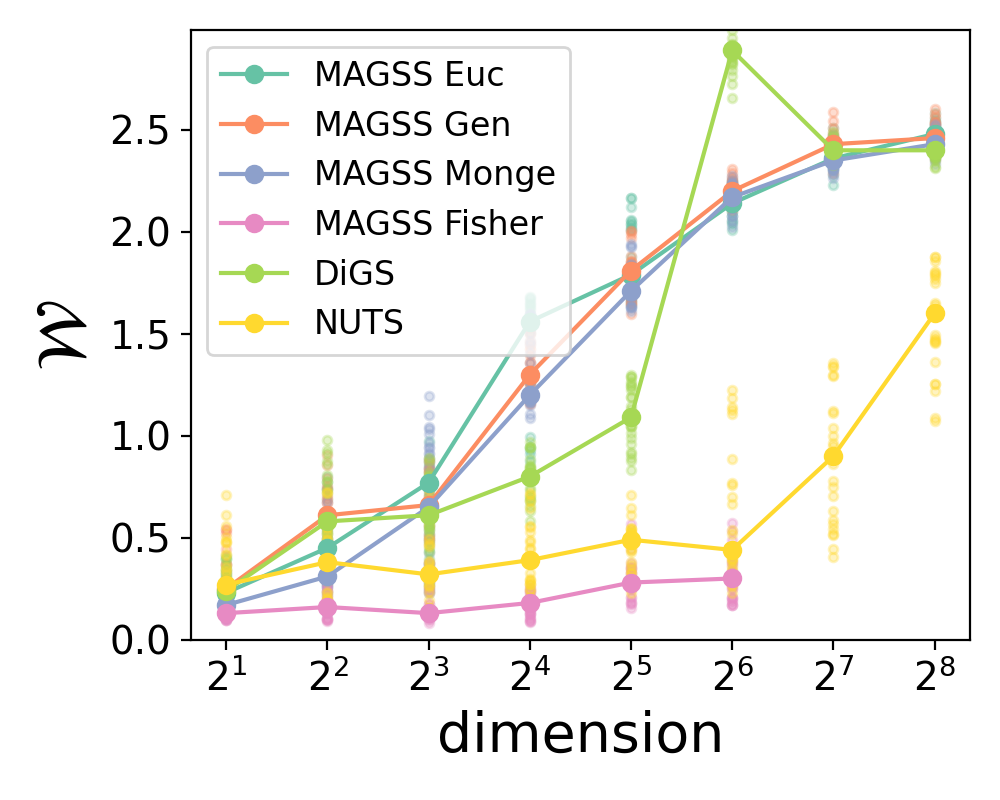
\includegraphics[width=\textwidth]{figs/paper2/rebutal/funnel_dims.png}
    \end{minipage}
    \hfill
    \begin{minipage}{0.32\textwidth}
        \centering
        {Rosenbrock}\\
        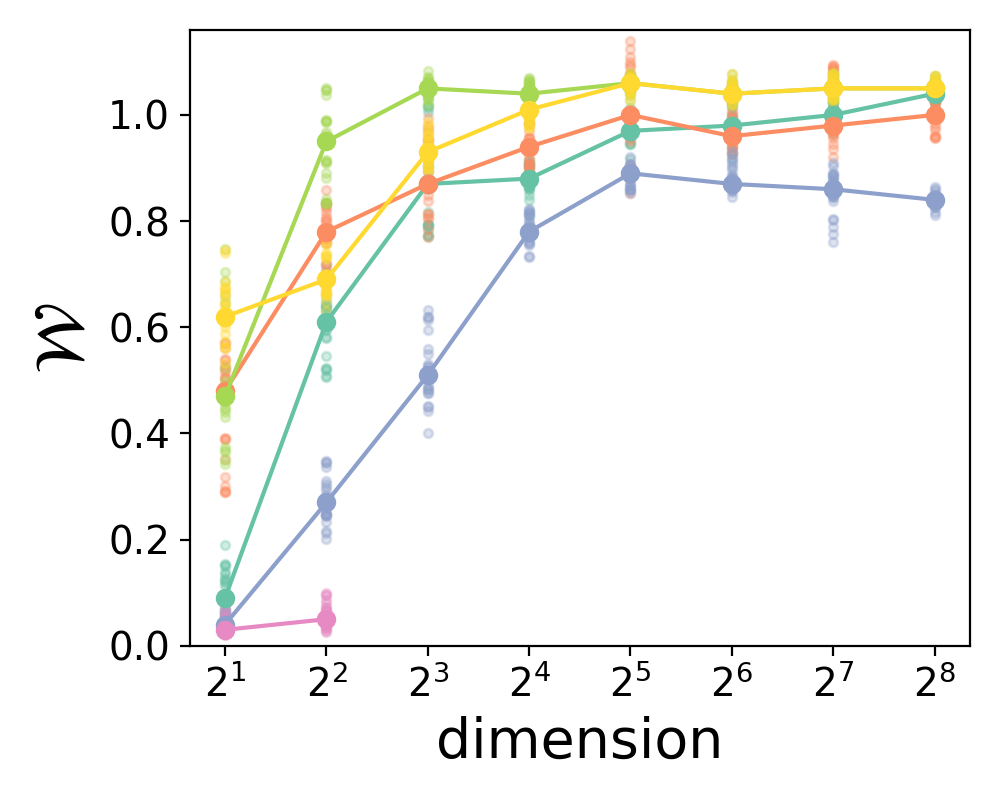
\includegraphics[width=\textwidth]{figs/paper2/rebutal/rosenbrock_dims.png}
    \end{minipage}
    \hfill
    \begin{minipage}{0.32\textwidth}
        \centering
        {Squiggle}\\
        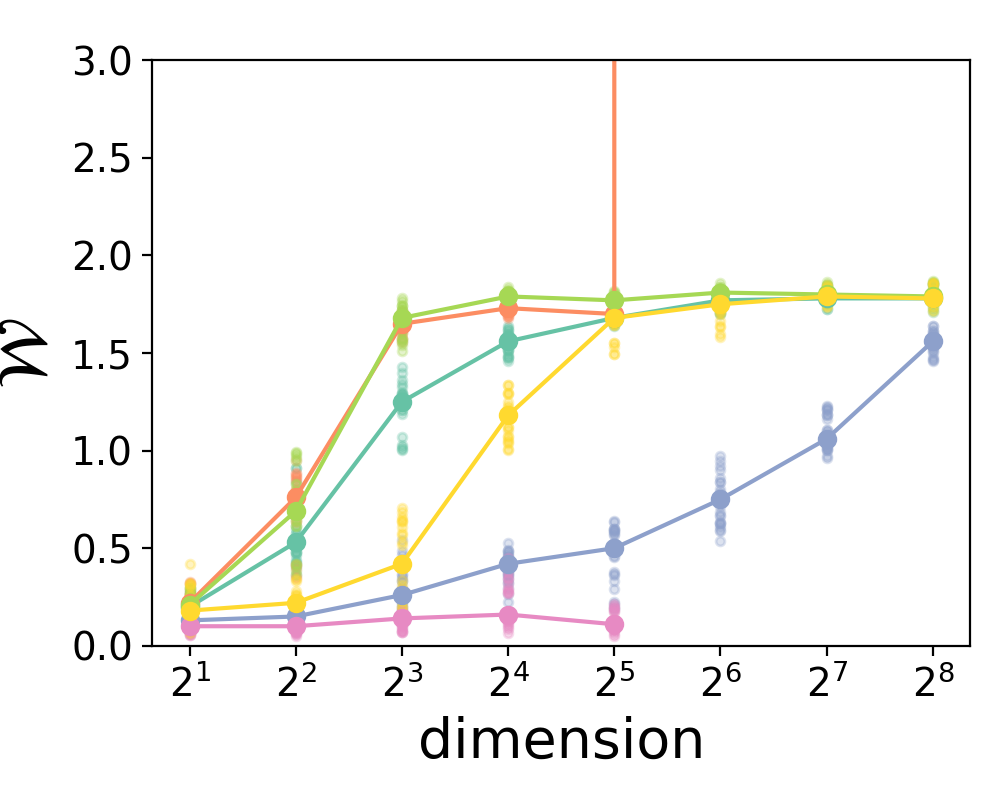
\includegraphics[width=\textwidth]{figs/paper2/rebutal/squiggle_dims.png}
    \end{minipage}
    \caption{Univariate sampling accuracy on different choice of Riemannian metric (1-Wasserstein distance, lower is better) for targets of varying dimensionality. The medians over 5 runs are connected with a line.}
    \label{fig:toydistdims}
\end{figure}

\paragraph{Highly multimodal target}
We consider the Allen-Cahn field system which has $2^D$ modes with $D=16$. This model has two global modes at $\boldsymbol{x} = \pm\boldsymbol{1}$, and multiple local modes at values $\boldsymbol{x} = (\pm 1,.., \pm 1)$. Table~\ref{tab:phifour} shows the results of the different sampling methods. 
Since there is no access to reference samples, we compute the Kernel Stein Discrepancy, but it is not trustworthy since it does not account for multimodality, the table also reports the percentage of samples such that $x_8\geq 0$ to see if the method was stuck on a single mode and the running time in seconds. MAGSS and DiGS are one order of magnitude slower than PT since they both rely on numerical integration.
Figure~\ref{fig:fieldsystem} shows that MAGSS explores the global and local modes, jumping the most frequently in between, while PT explores only the global modes and DiGS collapses to a single mode. A log-10 grid of parameters $\alpha^2, \lambda$ was tried, selecting the value based on the jump percentage. The inner sampler MALA stepsize was tuned to obtain an acceptance rate of approximately $60\%$. DiGS used $1000$ interpolation levels, ranging from $10^{-5}$ to $1-10^{-5}$. 
PT used $200$ temperatures on a geometric scale, with the smallest inverse temperature set to $10^{-5}$.

\begin{table}[t]
    \centering
    \caption{Allen-Cahn system model.}
\begin{tabular}{lllll}
\toprule
sampler &  KSD V-stat & $x_8>0$ & t(s) \\
\midrule
PT &   $0.13\pm0.04$ & $0.35$ & 6 \\
DiGS &   $0.13\pm0.05$ & $0.0$ & 157 \\
Meta-MAGSS  & $2.98\pm0.7$ & $0.33$ & 32 \\
\bottomrule
\end{tabular}    
    \label{tab:phifour}
\end{table}

\begin{figure}[t]
    \centering
    \begin{minipage}{0.32\linewidth}
        \centering
        {DiGS}\\
        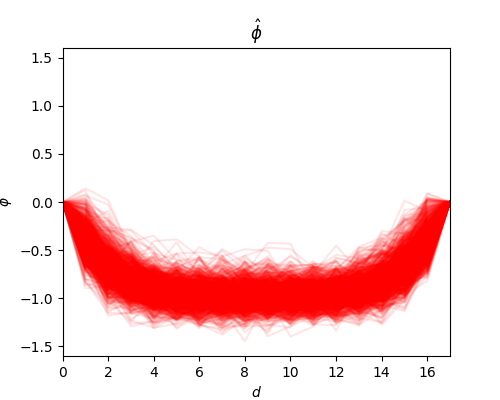
\includegraphics[width=\linewidth]{figs/paper2/rebutal/field_digs.png}
    \end{minipage}
    \hfill
    \begin{minipage}{0.32\linewidth}
        \centering
        {PT}\\
        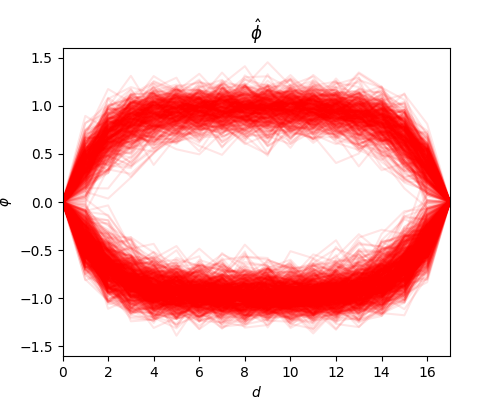
\includegraphics[width=\linewidth]{figs/paper2/rebutal/field_pt.png}
    \end{minipage}
    \hfill
    \begin{minipage}{0.32\linewidth}
        \centering
        {MAGSS}\\
        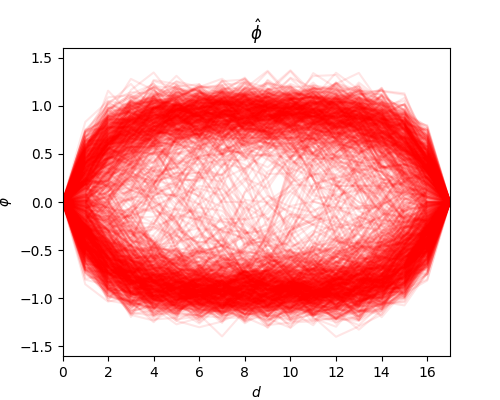
\includegraphics[width=\linewidth]{figs/paper2/rebutal/field_meta.png}
    \end{minipage}
    \caption{Samples from Allen-Cahn field system model with $2^{16}$ modes that zig-zag between $-1$ and $1$ on the y-axis over the $D=16$ values at the x-axis. Euclidean DiGS gets stuck in one mode, PT only explores two dominant modes with constant value over the x-axis, whereas Meta-MAGSS (inverse generative with $\lambda=10^{-6}$) explores also the modes that switch between the extremes.}
    \label{fig:fieldsystem}
\end{figure}


\paragraph{Sensitivity to the numerical integrator}
Here we study the effect of the choice of numerical integrator on a two dimensional 40-mode Gaussian  multimodal target for different values of $\alpha^2$ and $\lambda$ on a log-10 scale. We test integrators that are adaptive or fixed step-size and integrators with different order accurate solutions (see Figure~\ref{fig:gmm40}). 
The general trend is that as the inverse Monge and inverse generative metrics diverge from the Euclidean metric ($\alpha^2$ grows, $\lambda$ decreases), the system becomes stiffer and takes longer to integrate numerically. For the inverse Monge metric higher order and adaptive integrators work better, in practice we used Dopri5 in the other experiments because it has a good balance between the two. 
\begin{figure}[t]
    \centering
    \begin{minipage}{0.45\linewidth}
        \centering
        {Inverse generative metric}\\[0.5ex]
        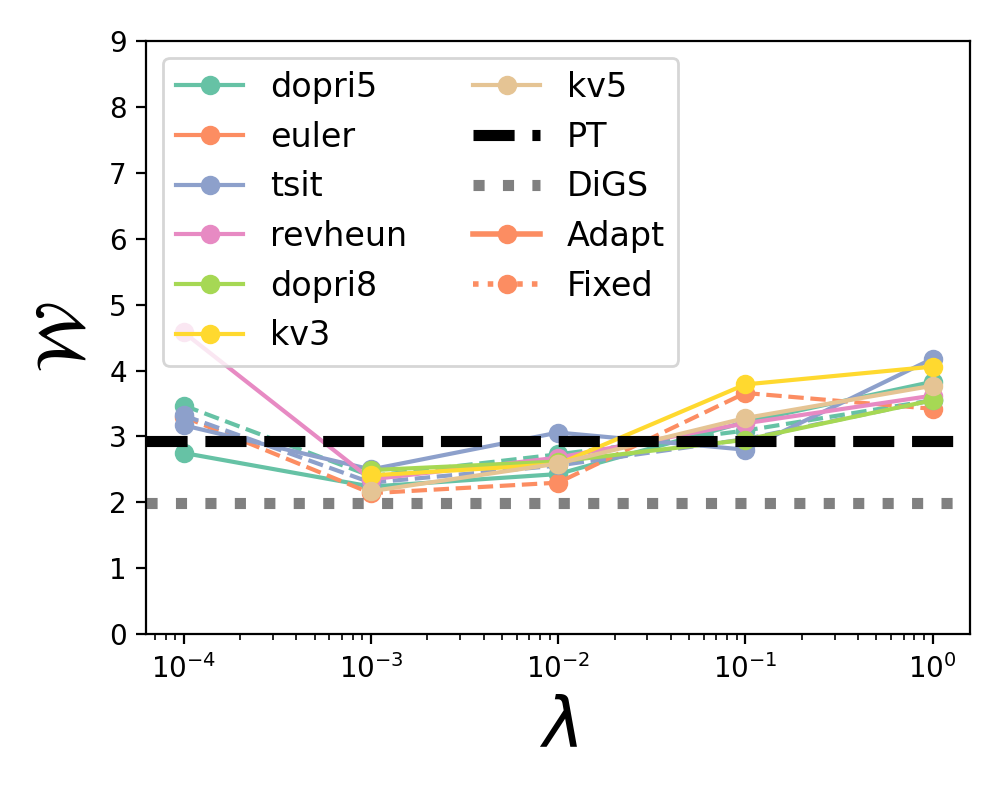
\includegraphics[width=\linewidth]{figs/paper2/gmm40/invGen_distances_mean_integrators.png}\\
        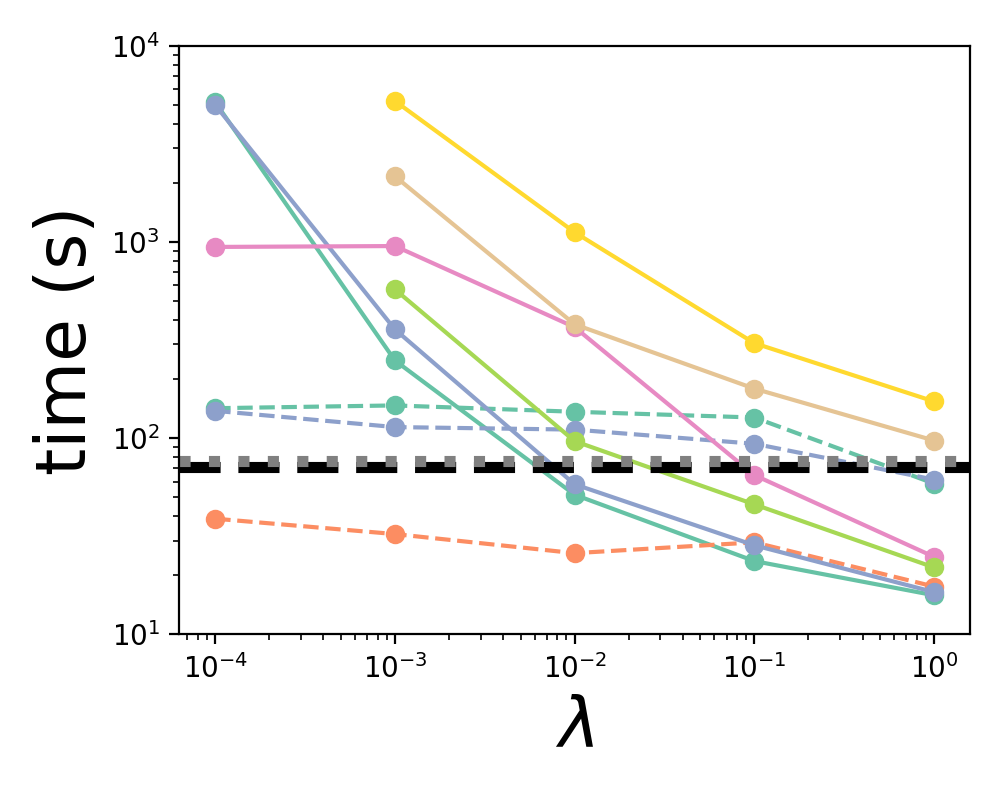
\includegraphics[width=\linewidth]{figs/paper2/gmm40/invGen_time_integrators.png}
    \end{minipage}
    \hfill
    \begin{minipage}{0.45\linewidth}
        \centering
        {Inverse Monge metric}\\[0.5ex]
        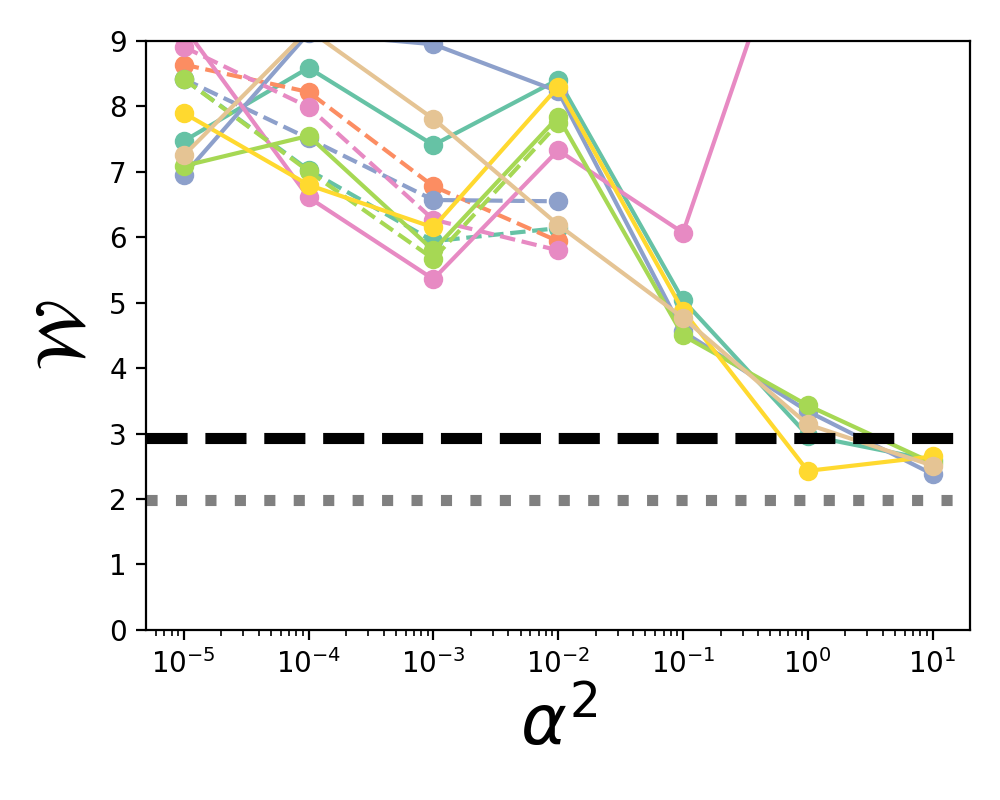
\includegraphics[width=\linewidth]{figs/paper2/gmm40/invMon_distances_mean_integrators.png}\\
        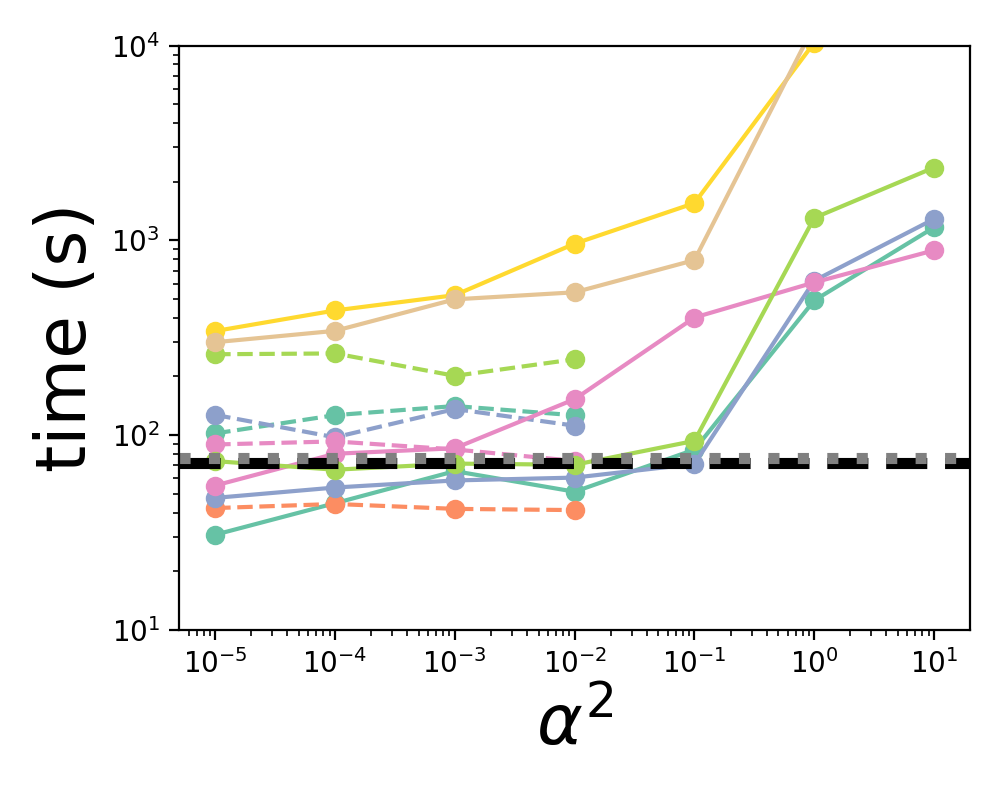
\includegraphics[width=\linewidth]{figs/paper2/gmm40/invMon_time_integrators.png}
    \end{minipage}
    \caption{Different numerical integrators for the 40 mode Gaussian mixture model. 
    The black dotted lines are PT and DiGS. Interpretation: the more the metric diverges from Euclidean (larger $\alpha^2$ and smaller $\lambda$) the more stiff the system is and the longer it takes to integrate. Generally, stiff systems benefit from adaptive integrators and produce more accurate samples.}
    \label{fig:gmm40}
\end{figure}
